\chapter{Настройка DNS-сервера BIND9}
\label{ch:practice}

\section{Настройка named.conf.options}

\begin{lstlisting}
nano /etc/bind/named.conf.options
\end{lstlisting}

Содержимое файла:
\begin{lstlisting}
options {
    directory "/var/cache/bind";
    forwarders { 8.8.8.8; };
    dnssec-validation auto;
    auth-nxdomain no;  # conform to RFC1035
    listen-on { 127.0.0.1; 192.168.N.1; };
};
\end{lstlisting}

Параметр \texttt{forwarders} задаёт DNS Google для внешних запросов;
\texttt{listen-on} ограничивает интерфейсы, на которых сервер принимает запросы:
localhost и LAN-адрес \texttt{192.168.\cfgLabStudentN.1}.

% — Скриншот: nano /etc/bind/named.conf.options с заполненным содержимым —
\begin{figure}[h]
  \centering
  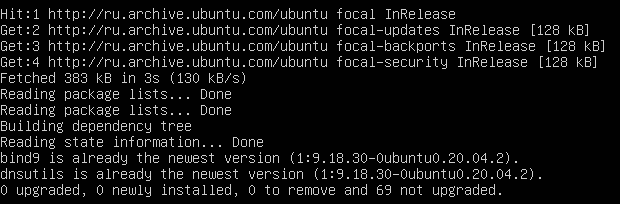
\includegraphics[width=0.85\textwidth]{img/05_named_conf_options}
  \caption{Файл \texttt{named.conf.options} — форвардер и listen-on}
  \label{fig:named_options}
\end{figure}

\section{Настройка named.conf.local}

\begin{lstlisting}
nano /etc/bind/named.conf.local
\end{lstlisting}

Содержимое файла:
\begin{lstlisting}
include "/etc/bind/rndc.key";
controls {
    inet 127.0.0.1 allow { localhost; } keys { rndc-key; };
};

zone "STUDENT.GROUP.local" IN {
    type master;
    file "/var/lib/bind/forward.db";
    allow-update { key rndc-key; };
};

zone "N.168.192.in-addr.arpa" IN {
    type master;
    file "/var/lib/bind/reverse.db";
    allow-update { key rndc-key; };
};
\end{lstlisting}

Файлы зон размещаются в \texttt{/var/lib/bind/}: BIND имеет туда права на запись,
что необходимо для DDNS-журналирования (\texttt{.jnl}-файлы).

% — Скриншот: nano /etc/bind/named.conf.local с описанием зон —
\begin{figure}[h]
  \centering
  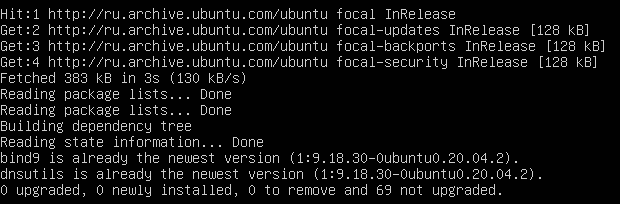
\includegraphics[width=0.85\textwidth]{img/06_named_conf_local}
  \caption{Файл \texttt{named.conf.local} — описание прямой и обратной зон}
  \label{fig:named_local}
\end{figure}

\section{Создание файла прямой зоны}

\begin{lstlisting}
nano /var/lib/bind/forward.db
\end{lstlisting}

\begin{lstlisting}
$TTL 86400
STUDENT.GROUP.local. IN SOA SERVERHOSTNAME.STUDENT.GROUP.local. admin.STUDENT.GROUP.local. (
    20110103 ; Serial
    604800   ; Refresh
    86400    ; Retry
    2419200  ; Expire
    604800 ) ; Negative Cache TTL

@ IN NS  SERVERHOSTNAME.STUDENT.GROUP.local.
@ IN A   192.168.N.1
localhost       IN A 127.0.0.1
SERVERHOSTNAME  IN A 192.168.N.1
\end{lstlisting}

% — Скриншот: nano /var/lib/bind/forward.db —
\begin{figure}[h]
  \centering
  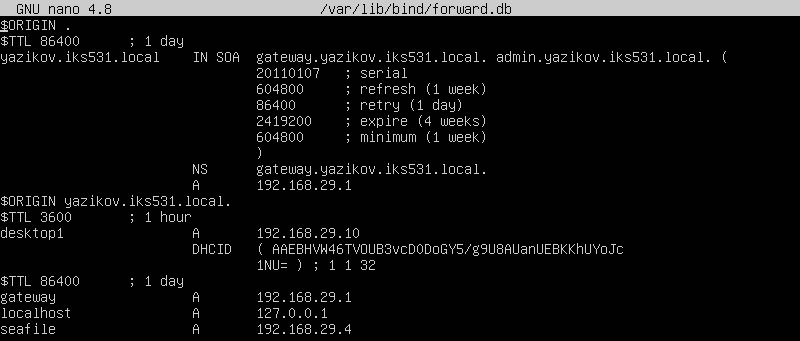
\includegraphics[width=0.85\textwidth]{img/07_forward_db}
  \caption{Файл прямой зоны \texttt{forward.db}}
  \label{fig:forward_db}
\end{figure}

\section{Создание файла обратной зоны}

\begin{lstlisting}
nano /var/lib/bind/reverse.db
\end{lstlisting}

\begin{lstlisting}
$TTL 86400
N.168.192.in-addr.arpa. IN SOA STUDENT.GROUP.local. STUDENT.GROUP.local. (
    20110104 ; Serial
    10800    ; Refresh
    3600     ; Retry
    604800   ; Expire
    3600 )   ; Minimum

@ IN NS SERVERHOSTNAME.STUDENT.GROUP.local.
1   IN PTR STUDENT.GROUP.local.
1   IN PTR SERVERHOSTNAME.STUDENT.GROUP.local.
\end{lstlisting}

% — Скриншот: nano /var/lib/bind/reverse.db —
\begin{figure}[h]
  \centering
  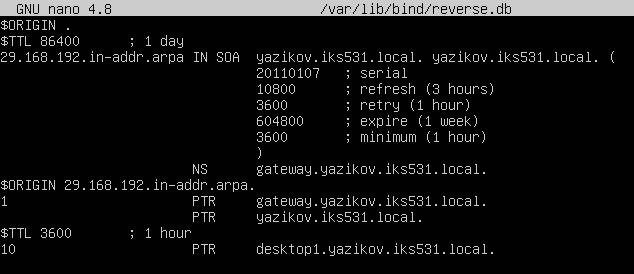
\includegraphics[width=0.85\textwidth]{img/08_reverse_db}
  \caption{Файл обратной зоны \texttt{reverse.db}}
  \label{fig:reverse_db}
\end{figure}

\section{Проверка конфигурации и перезапуск BIND9}

\begin{lstlisting}
named-checkconf
named-checkzone STUDENT.GROUP.local /var/lib/bind/forward.db
named-checkzone N.168.192.in-addr.arpa /var/lib/bind/reverse.db
systemctl restart bind9
\end{lstlisting}

% — Скриншот: вывод named-checkconf и named-checkzone (нет ошибок) —
\begin{figure}[h]
  \centering
  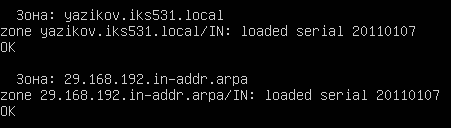
\includegraphics[width=0.85\textwidth]{img/09_named_checkconf}
  \caption{Проверка конфигурации BIND9 без ошибок}
  \label{fig:named_check}
\end{figure}

\section{Настройка netplan на gateway}

\begin{lstlisting}
nano /etc/netplan/00-installer-config.yaml
\end{lstlisting}

\begin{lstlisting}
network:
  version: 2
  renderer: networkd
  ethernets:
    enp0s3:
      dhcp4: no
      addresses: [10.0.2.15/24]
      gateway4: 10.0.2.2
    enp0s8:
      dhcp4: no
      addresses: [192.168.N.1/24]
      nameservers:
        addresses: [192.168.N.1]
        search: [STUDENT.GROUP.local]
\end{lstlisting}

\begin{lstlisting}
netplan apply
\end{lstlisting}

% — Скриншот: nano /etc/netplan/00-installer-config.yaml с nameservers —
\begin{figure}[h]
  \centering
  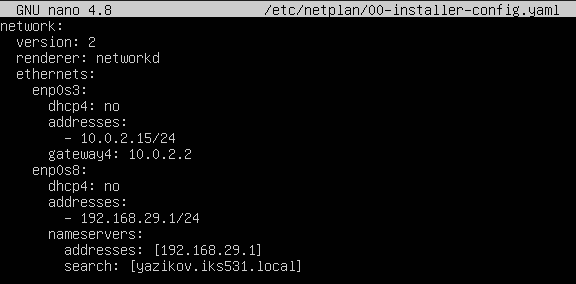
\includegraphics[width=0.85\textwidth]{img/10_netplan_gateway}
  \caption{Файл \texttt{netplan} gateway — DNS указан на localhost}
  \label{fig:netplan_gw}
\end{figure}

\section{Проверка DNS}

\begin{lstlisting}
nslookup SERVERHOSTNAME
nslookup 192.168.N.1
\end{lstlisting}

% — Скриншот: вывод nslookup SERVERHOSTNAME (успешное разрешение) —
\begin{figure}[h]
  \centering
  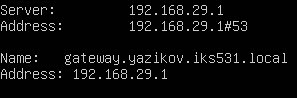
\includegraphics[width=0.85\textwidth]{img/11_nslookup_forward}
  \caption{Прямое разрешение имени через \texttt{nslookup}}
  \label{fig:nslookup_fwd}
\end{figure}

% — Скриншот: вывод nslookup 192.168.N.1 (обратное разрешение) —
\begin{figure}[h]
  \centering
  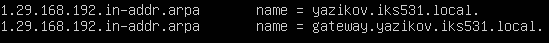
\includegraphics[width=0.85\textwidth]{img/12_nslookup_reverse}
  \caption{Обратное разрешение IP через \texttt{nslookup}}
  \label{fig:nslookup_rev}
\end{figure}

\section{Настройка DDNS}

\subsection{Копирование ключа RNDC}

\begin{lstlisting}
cp -Rr /etc/bind/rndc.key /etc/dhcp/ddns-keys/
\end{lstlisting}

\subsection{Обновление dhcpd.conf}

\begin{lstlisting}
nano /etc/dhcp/dhcpd.conf
\end{lstlisting}

Полная конфигурация с DDNS:
\begin{lstlisting}
include "/etc/dhcp/ddns-keys/rndc.key";

ddns-updates on;
ddns-update-style standard;
ddns-domainname "STUDENT.GROUP.local";

zone STUDENT.GROUP.local. {
    primary 192.168.N.1;
    key rndc-key;
}

zone N.168.192.in-addr.arpa. {
    primary 192.168.N.1;
    key rndc-key;
}

authoritative;

subnet 192.168.N.0 netmask 255.255.255.0 {
    range 192.168.N.10 192.168.N.254;
    option domain-name-servers 192.168.N.1;
    option domain-name "STUDENT.GROUP.local";
    option routers 192.168.N.1;
    option broadcast-address 192.168.N.255;
    default-lease-time 604800;
    max-lease-time 604800;
}
\end{lstlisting}

% — Скриншот: nano /etc/dhcp/dhcpd.conf (блок ddns + zone) —
\begin{figure}[h]
  \centering
  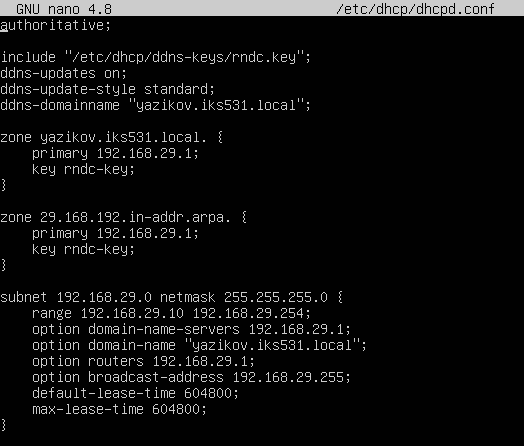
\includegraphics[width=0.85\textwidth]{img/13_dhcpd_conf_ddns}
  \caption{Файл \texttt{dhcpd.conf} — секция DDNS}
  \label{fig:dhcpd_ddns}
\end{figure}

\subsection{Перезапуск сервисов}

\begin{lstlisting}
systemctl restart bind9
service isc-dhcp-server restart
service isc-dhcp-server status
\end{lstlisting}

% — Скриншот: service isc-dhcp-server status (active running) —
\begin{figure}[h]
  \centering
  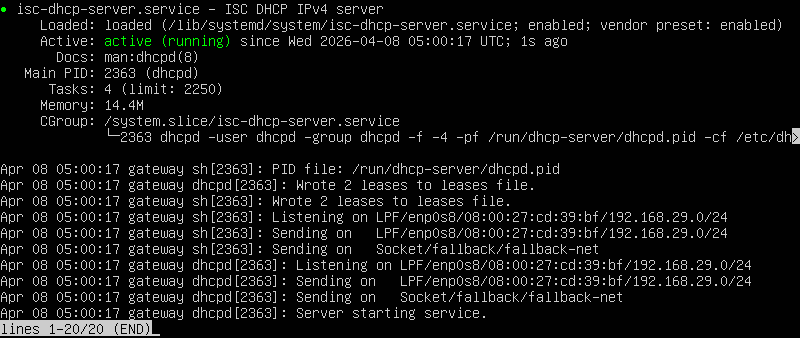
\includegraphics[width=0.85\textwidth]{img/14_dhcp_status}
  \caption{Статус сервиса \texttt{isc-dhcp-server} — active (running)}
  \label{fig:dhcp_status}
\end{figure}

\subsection{Проверка DDNS}

После подключения Desktop к сети и получения IP-адреса по DHCP
проверяем автоматическую регистрацию в DNS:

\begin{lstlisting}
nslookup DESKTOPNAME01
tail -40 /var/log/syslog
\end{lstlisting}

% — Скриншот: вывод nslookup DESKTOPNAME01 (IP получен от DNS) —
\begin{figure}[h]
  \centering
  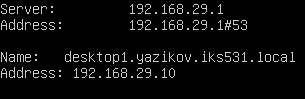
\includegraphics[width=0.85\textwidth]{img/15_nslookup_desktop}
  \caption{Разрешение имени Desktop-клиента через DDNS}
  \label{fig:nslookup_desktop}
\end{figure}

% — Скриншот: tail /var/log/syslog (записи DDNS update succeeded) —
\begin{figure}[h]
  \centering
  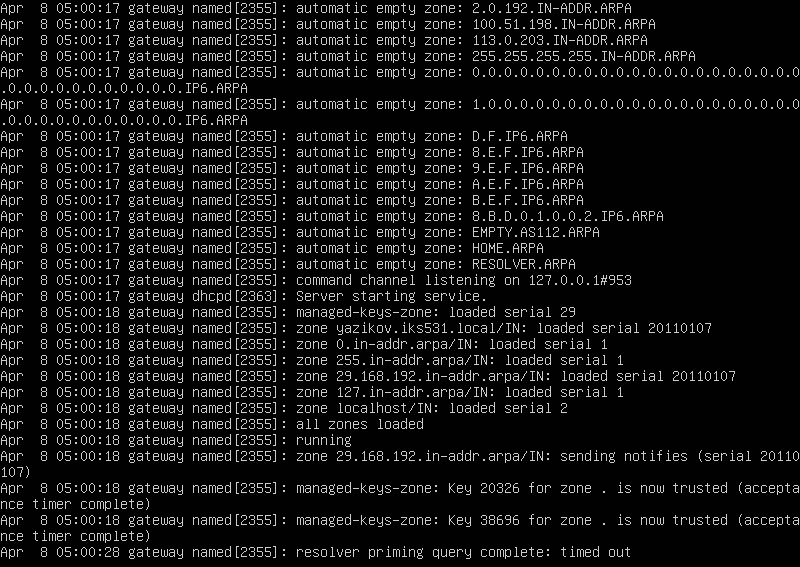
\includegraphics[width=0.85\textwidth]{img/16_syslog_ddns}
  \caption{Лог \texttt{syslog} — успешное DDNS-обновление}
  \label{fig:syslog_ddns}
\end{figure}

\endinput
